\documentclass{swfcthesis}
\usepackage{makecell}


\renewcommand{\acknowledgmentspage}{% Acknowledgments page  
  \phantomsection%
  \addcontentsline{toc}{chapter}{Acknowledgments}
  \chapter*{Acknowledgments}

  I would like to thank my supervisor Mr. WANG Xiaolin for his continuous support of my
  four years undergraduate study. I am extremly thankful to him for sharing expertise, and
  sincere and valuable guidance and encouragement extended to me.
    
  What I most want to thank is my girlfriend. She tolerated me when I finished this
  graduation project many nights did not accompany her, gave me support, encouraged me,
  and did not complain. So I would like to name this simple operating system as RongOS. Rong
  is the last word of her name. Thank you, my dearest.
  
  My special thanks to a great company - Google, I think I need to thank you in this very
  formal place in my graduation thesis. Every time you gave me a lot of help, the
  knowledge and other abilities I learned from you will have a profound impact on my
  future life. I am grateful for every search, because I know you will give me the results
  I want. Without you, this paper cannot be completed. Thank you.
    
}

\renewcommand{\advisorinfopage}{% Advisor info page
  \phantomsection%
  \addcontentsline{toc}{chapter}{Supervisor}
  \chapter*{Supervisor}
  Xiaolin WANG (Mr.), 49 years old, got his MSc degree at University of Greenwich in
  UK\@. Currently he's been working as a lecturer at the School of Big Data and
  Intelligence Engineering, Southwest Forestry University in China, teaching Linux,
  Operating Systems, and Computer Networking.
  \clearpage}

\renewcommand{\contentsname}{Contents}
\renewcommand{\listfigurename}{List of Figures}
\renewcommand{\listtablename}{List of Tables}
\renewcommand{\figurename}{Fig.}
\renewcommand{\tablename}{Table}
\renewcommand{\listingscaption}{Code} % used by minted
\renewcommand{\listoflistingscaption}{List of Codes}

\addbibresource{thesis.bib}

\begin{document}

\Title{RongOS --- 一个简单操作系统的设计与实现}
\Author{蒲启元}
\Advisor{王晓林}
\AdvisorTitle{讲师}
\Month{六}
\Year{二〇一八}

\Subject{计算机科学与技术专业} %专业名称(比如 电子信息工程专业)

\Abstract{操作系统管理着计算机的硬件和软件资源,它是向上层应用软件提供服务(接口)的核心系
  统软件,这些服务包括进程管理,内存管理,文件系统,网络通信,安全机制等。操作系统的设计与
  实现则是软件工业的基础。为此,在国务院提出的《中国制造2025》中专门强调了操作系统的开
  发\cite{china_2025}。但长期以来,操作系统核心开发技术都掌握在外国人手中,技术受制,对于我
  们的软件工业来说很不利。本项目从零开始设计开发一个简单的操作系统,包括boot loader,中断,
  内存管理,图形接口,多任务等功能模块,以及能运行在这个系统之上的几个小应用程序。尽管这
  个系统很简单,但它是自主开发操作系统的一次尝试。}

\Keywords{操作系统,进程,内存,中断,boot loader}

\enTitle{RongOS --- A simple OS implementation}

\enAuthor{Qiyuan PU}

\enAbstract{Operating system manages the hardware and software resources in a running
  computer system. It is the core of any modern software system and provides services
  (interfaces) to upper layer applications. The services it provides include process
  management, memory management, file system, network communication, security mechanism
  and more. Operating system development is the foundation and core of software
  industry. Therefore, \emph{Made in China 2025} emphasizes the development of operating
  system that put forward by The State Council of China. For long time, however, the OS
  kernel development technology is dominated by foreigners. This technical limitation is
  detrimental to the development of our software industry. In this project, we presents a
  simple operating system which includes a boot loader, interrupt services, memory
  management functions, a graphic interface, and multi-process management functions. Also,
  some trivial user-level applications are provided for system testing purpose. This
  simple toy OS is an experimental trial for developing an operating system from scratch.}

\enKeywords{operating system, boot loader, interrupt, process management, memory management}

%%% 下面六行不要动!
\makepreliminarypages% 封面
\frontmatter          
\tableofcontents     % 目录
\listoffigures       % 插图目录
\listoftables        % 表格目录
\listoffixmes{}

\mainmatter{}

\chapter{Introduction}
This section will introduce the purpose and current status of the operating system
research. The setup of the development environment will also be presented here.


\section{Background}

Contemporary software systems are beset by problems that create challenges and
opportunities for broad new OS research. There are five areas could improve user
experience including dependability, security, system configuration, system extension, and
multiprocessor programming.

The products of forty years of OS research are sitting in everyone's desktop computer,
cell phone, car, etc., and it is not a pretty picture.  Modern software systems are
broadly speaking complex, insecure, unpredictable, prone to failure, hard to use, and
difficult to maintain. Part of the difficult is that good software is hard to write, but
in the past decade, this problem and more specific shortcomings in systems have been
greatly exacerbated by increased networking and embedded systems, which placed new demands
that existing architectures struggled to meet. These problems will not have simple
solutions, but the changes must be pervasive, starting at the bottom of the software
stack, in the operating system.

The world needs broad operating system research. Dependability, security, system
configuration, system extension, and multi-processor programming illustrate areas were
contemporary operating systems have failed to meet the software challenges of the modern
computing environment\cite{hunt2005broad}.


\section{Preliminary Works}

\subsection{Development Environment}

\begin{description}
\item[OS platform:] Debian 9, Linux kernel 4.12.0-1-amd64
\item[Editor:] GNU Emacs 25.2.2
\item[Run time VM:] QEMU emulator 2.8.1
\item[Assembler:] Nask
\item[Compiler:] CC1(Based on gcc)
\item[Debugger:] GNU gdb 7.12
\item[Version Control:] git 2.15
\end{description}

\subsection{Tools}

Some tools were used to develop RongOS, See \emph{tools}\footnote{\url{https://github.com/Puqiyuan/RongOS/tree/master/z_tools}}. Note that
these tools are Windows executable. Please install wine if you want to run these tools on
Linux. In these tools, the most important ones are:

\begin{description}
\item[nask.exe:] the assembler, a modified version of NASM\cite{30_os}
\item[cc1:] the C compiler
\end{description}

\subsection{Platform Setup}

The development platform (mainly the Debian system) was set up by following the
\emph{Debian Installation
  tutorial}\footnote{\url{http://cs2.swfc.edu.cn/~wx672/lecture_notes/linux/install.html}}. The
main steps include:
\begin{enumerate}
\item Installing the base Debian system;
\item Installing necessary software tools, such as emacs, web browser, qemu, wine, etc.;
\item Cloning configuration files by following the tutorial mentioned above;
\item Some more fine tweaks to satisfy my personal needs.
\end{enumerate}

\subsubsection{Qemu}

QEMU is a generic and open source machine emulator and virtualizer\cite{wiki:qemu}. In
this project, QEMU was used as the test bed.

Installing QEMU for my x86\_64 architecture can be easily done by executing the following
command:
\begin{verbatim}
     $ sudo apt-get install qemu-system-x86_64
\end{verbatim}

\subsubsection{Wine}

Wine (originally an acronym for ``Wine Is Not an Emulator'') is a compatibility layer
capable of running Windows applications on several POSIX-compliant operating systems, such
as Linux, macOS, and BSD\cite{wiki:wine}.

Because the tools I used in this project are in Windows executable format, so on Debian system,
Wine is needed to be installed:

\begin{verbatim}
     $ sudo apt-get update
     $ sudo apt-get install wine
\end{verbatim}

\subsubsection{Debian i386 support}

On 64-bit systems you need to enable multi-arch support for running 32-bit Windows
applications (many modern apps are still 32-bit, also for large parts of the Windows
subsystem itself). Our development tools were 32-bit Windows applications, so we needed to
have i386 support for our 64-bit Linux system.

\begin{verbatim}
     $ sudo dpkg --add-architecture i386
     $ sudo apt-get update
\end{verbatim}

\iffalse %%%%%%%%%%%%%%%%%%%%%%%%%%%%%%%%%%%%%%%%%%%%%%%%%%%%%%%%%%%%%%%%%%%%%%%%%%%%%%%%%%%%%%%%%
%\chapter{Leading Knowledge}
%\label{cha:leading-knowledge-1}

%\section{Layers}
%\label{sec:layers}

%\section{Memory Management}
%\label{sec:memory-management}

%\subsection{Overview}
%\label{sec:overview}

%\subsection{Round Down/Up and Page Size}
%\label{sec:round-downup-page}


%\section{Mouse}
%\label{sec:mouse}

%\section{The Leap --- Road to the 32 Bit Mode}
%\label{sec:leap-road-32}

%\section{Data Structure}
%\label{sec:data-structure}

%\section{Programmable Interrupt Controller}

\section{C Language Basic}

\section{Segments and Descriptors}
The so-called segmentation is to divide a total of 4 GB of memory into many blocks in its
own way. The start address of each block is treated as 0.

In this way, in order to represent a segment, the following information is required:
\begin{itemize}
\item The size of the segment
\item Where is the starting address of the segment
\item Segment management properties
\end{itemize}

All this information is represented by 8 bytes(64 bits). But the register used to specify
the segment is only 16 bits. Therefore, the segment selector is stored in the segment
register, and the segment management information(the above three information) is
referenced by the segment selector. Although the segment register has 16 bits, only high 13
bits are available due to the CPU design. Therefore, the segment selector is in the range
of 0 to 8191. In total, there are 8192 segments, and a total of 8192 × 8 = 65536(64KB) bytes are
required to store the management information of these segments. This 64-byte message is
called GDT. Obviously, the CPU does not have such a large storage capacity. So store this
information somewhere in memory. A special register in the CPU is GDTR(global descriptor
table register). This register is used to reference the GDT address in memory and record
how many valid segments are set.



\section{Instruction Set}

An instruction set architecture (ISA) is an abstract model of a computer. It is also
referred to as architecture or computer architecture. An ISA defines everything a machine
language programmer needs to know in order to program a computer.

An ISA may be classified in a number of different ways. A common classification is by
architectural complexity. A complex instruction set computer (CISC) has many specialized
instructions, some of which may only be rarely used in practical programs. A reduced
instruction set computer (RISC) simplifies the processor by efficiently implementing only
the instructions that are frequently used in programs, while the less common operations
are implemented as subroutines, having their resulting additional processor execution time
offset by infrequent use.

On traditional architectures, an instruction includes an opcode that specifies the
operation to perform, such as add contents of memory to register—and zero or more operand
specifiers, which may specify registers, memory locations, or literal data\cite{wiki:isa}.

This simple RongOS is based on x86 architecture, the following instructions are commonly
used in programming RongOS:%

\begin{description}
\item[db:] the abbreviation of define byte, write a byte, also 8 bits to file.
\item[resb:] the abbreviation of reserve byte, reserved bytes and filling \texttt{0x00} in these reserved space.
\item[dw:] the abbreviation of define word, write two bytes, also 16 bits to file.
\item[dd:] the abbreviation of define double-word, write four bytes, also 32 bits to file.
\item[org:] load the program to specified address.
\item[jmp:] jump to another instruction.
\item[mov:] assign the right value to left variable.
\item[jc:] the abbreviation of jump if carry, it means if carry flag is 1, jump.
\item[jnc:] jump if not carry.
\item[jae:] jump if above or equal.
\item[jbe:] jump if below or equal.
\item[jb:] jump if below.
\item[equ:] equ is the abbreviation of equal.
\item[ret:] end of function, return.
\item[in:] get signal from device.
\item[out:] send signal to device.
\item[cli:] clear interrupt flag, set it to 0.
\item[sti:] set interrupt flag, set it to 1.
\item[pushfd:] push flags double-word.
\item[popfd:] pop flags double-word.
\item[lgdt:] load content from specified memory to initialize GDT (global descriptor table)
  register.
\item[lidt:] load content from specified memory to initialize IDT (interrupt descriptor
  table) register.
\end{description}

\section{x86 Registers}

In computer architecture, a processor register is a quick accessible location available
to a computer's central processing unit (CPU). Registers usually consist of a small amount
of fast storage, although some registers have specific hardware functions, and may be
read-only or write-only.  Almost all computers, whether load/store architecture or not,
load data from a larger memory into registers where it is used for arithmetic operations
and is manipulated or tested by machine instructions. Manipulated data is then often
stored back to main memory, either by the same instruction or by a subsequent one. Modern
processors use either static or dynamic RAM as main memory, with the latter usually
accessed via one or more cache levels\cite{wiki:registers}.

Processor registers are normally at the top of the memory hierarchy, and provide the
fastest way to access data. The term normally refers only to the group of registers that
are directly encoded as part of an instruction, as defined by the instruction
set. Registers are normally measured by the number of bits they can hold, for example, an
``8-bit register'' or a ``32-bit register''. For x86 architecture, the following registers
exist, see 3.4.1 and 3.4.2 \cite{guide2011intel}:

\begin{multicols}{3}
  \begin{description}
  \item[ax:] accumulator
  \item[bx:] base
  \item[cx:] counter
  \item[dx:] data
  \item[bl:] base low
  \item[al:] accumulator low
  \item[cl:] counter low
  \item[dl:] data low
  \item[bh:] base high
  \item[ah:] accumulator high
  \item[ch:] counter high
  \item[dh:] data high
  \item[sp:] stack pointer
  \item[bp:] base pointer
  \item[si:] source index
  \item[di:] destination index
  \item[es:] extra segment
  \item[cs:] code segment
  \item[ss:] stack segment
  \item[ds:] data segment
  \item[fs:] no name
  \item[gs:] no name
  \end{description}
\end{multicols}

Among these registers, \texttt{bx, bp, si} and \texttt{di} can be used to specify the
address of memory. But \texttt{ax, cx, dx} and \texttt{sp} can not. When \emph{mov}
instruction is used, the number of bits of source number should be the same with
destination operand.

\begin{description}
\item[16-bit registers:] \texttt{ax, cx, dx, bx, sp, bp, si, di, es, cs, ss, ds}, and \texttt{fs}.
\item[8-bit registers] \texttt{al, cl, dl, bl, ah, ch, dh}, and \texttt{bh}.
\end{description}
Actually, as shown in Fig.~\ref{fig:regs}, all these 8-bit registers are parts of
corresponding 16-bit registers.

\begin{figure}[!htbp]
  \centering
  \begin{center}
    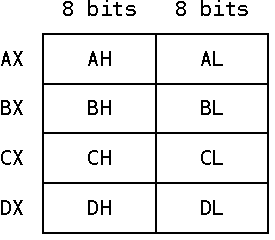
\includegraphics[width=.4\textwidth]{registers}
  \end{center}
  \caption{x86 registers}
  \label{fig:regs}
\end{figure}

\section{Interrupt Call}

BIOS interrupt calls perform hardware control or I/O functions requested by a program,
return system information to the program, or do both. A key element of the purpose of BIOS
calls is abstraction. The BIOS calls perform generally defined functions, and the specific
details of how those functions are executed on the particular hardware of the system are
encapsulated in the BIOS and hidden from the program\cite{wiki:bios-int}. The interrupt
calls are commonly used in RongOS are listed in Table~\ref{tbl:intcall}.

\begin{table}[!ht]
  \centering\tabulinesep=2mm
  \begin{tabu}{X[l,m,-1]X[l,m]X[-1,l,m]X[-1,l,m]}
    \tabucline-\rowfont\bfseries
    Interrupt\par{}Number & Register Parameter & Return Value & Function\\ \tabucline-
    0x10 &
    ah=0x0e(write character in tty mode)\par{}
    al=character code\par{}
    bh=0, bl=colorcolor& null & video services \\\tabucline-
    0x13 &
    ah=0x02(read sectors)\par{}
    ah=0x03(write sectors)\par{}
    ah=0x04(verify sectors)\par{}
    ah=0x0c(seek to specified track)\par{}
    al=number of sectors processing\par{}
    ch=cylinder \& 0xff  cl=sector number\par{}
    dh=header number dl=driver number\par{}
    es:bx=buffer address &
    FLACS.CF=0\par{}
    no error, ah = 0\par{}
    FLAGS.CF=1\par{}
    error, ah=error number\par{}& disk services \\ \tabucline-
  \end{tabu}
  \caption{RongOS interrupt calls}\label{tbl:intcall}
\end{table}

\section{Memory Map}

In the boot process, a memory map is passed on from the firmware in order to instruct an
operating system kernel about memory layout. It contains the information regarding the
size of total memory, any reserved regions and may also provide other details specific to
the
architecture\footnote{http://hypervsir.blogspot.com/2014/09/approach-to-retrieving-bios-memory-map.html}. For
loading RongOS to memory, the memory layout should be clarified as in
Table~\ref{tbl:memlayout}.


\begin{table}[!ht]
  \centering\tabulinesep=2mm
  \begin{tabu}{%
      >{\texttt\bgroup}r<{\egroup}@{\,--\,}>{\texttt\bgroup}l<{\egroup}%
      >{\texttt\bgroup}r<{\egroup}@{\,--\,}>{\texttt\bgroup}l<{\egroup}%
      >{\texttt\bgroup}l<{\egroup}l}%
    \tabucline-\rowfont\bfseries%
    \multicolumn{2}{l}{Range (in hexadecimal)} &%
    \multicolumn{2}{l}{Range (in decimal)} &%
    \multicolumn{1}{l}{Size (in bytes)} & Usage \\ \tabucline-
    0000 & 03ff & 0000 & 1023 & 1024 &  interrupt vector table \\ 
    0400 & 04ff & 1024 & 1279 & 256 & BIOS data area \\ 
    0500 & 051f & 1280 & 1311 & 32 & Reserved \\ 
    0520 & 7bff & 1312 & 31743 & 30432 & conventional memory \\ 
    7c00 & 7dff & 31744 & 32255 & 512 & master boot record \\ 
    7e00 & 9ffff & 32256 & 655359 & 623104 & conventional memory \\ 
    a0000 & affff & 655360 & 720895 & 64K & VGA graphics RAM \\ 
    b0000 & b7fff & 720896 & 753663 & 32K & monochrome text mode \\ 
    b8000 & bffff & 753664 & 786431 & 32K & color text mode \\ 
    c0000 & c7fff & 786432 & 819199 & 32K & VGA video ROM \\ 
    c8000 & cbfff & 819200 & 835583 & 16K & IDE hard drive \\ 
    cc000 & cffff & 835584 & 851967 & 16K & optional adapter \\ \tabucline-
  \end{tabu}
  \caption{RongOS Memory Layout}\label{tbl:memlayout}
\end{table}

\section{Floppy Disk}

There are many ways to boot an operating system, from hard disk, USB, floppy disk, etc.
The structure of floppy disk is simple and for this simple operating system it's enough.

Fig.~\ref{fig:flpy1.png} shows the inside of a floppy disk:
\begin{figure}[!ht]
  \centering
  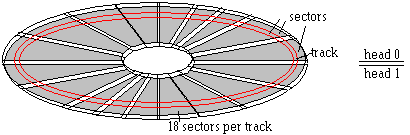
\includegraphics[width=.5\textwidth]{../figs/bootLoader/flpy1.png}
  \caption{Floppy disk structure}
  \label{fig:flpy1.png}
\end{figure}

A floppy disk, also called a floppy, diskette, or just disk, is a type of disk storage
composed of a disk of thin and flexible magnetic storage medium, sealed in a rectangular
plastic enclosure lined with fabric that removes dust particles. Floppy disks are read and
written by a floppy disk drive (FDD)\cite{wiki:floppy}.

For 3.5 inch HD floppy,  There are 80 cylinders from the outermost to
the core on each side, numbering 0, 1, \ldots, 79. The head can assign be 0 or 1,
representing two sides of floppy. When specify head number and cylinder number, forming a
ring, named track in jargon. The track is large so we divide it to 18 small parts, named
sector. A sector can store 512 byte. So the capacity of a floppy is:

\[18 \times 80 \times 2 \times 512 = 1474560\,Byte = 1440\,KiB\]

\fi %%%%%%%%%%%%%%%%%%%%%%%%%%%%%%%%%%%%%%%%%%%%%%%%%%%%%%%%%%%%%%%%%%%%%%%%%%%%%%%%%%%%%%%%%%%%%%%%


\chapter{Design}

This chapter describes the design issues in the entire software system, including system startup,
the kernel, APIs, and some applications.


\section{Top Level Design}

As shown in Fig.~\ref{fig:top-level} shown, all applications require services from the
operating system through a set of function calls. This set of functions provided by the OS
kernel is usually called \emph{system calls}. However, the user applications do not invoke
these system calls directly. Instead, they call the API library functions. The process in
which the API invokes a system call and hands over processing to the kernel is called
\emph{trapping}.

Within the kernel, there are some important software modules working to keep the system
running well. The process control subsystem provides graphics processing, CPU scheduling,
and memory management functions for processes. \fxerror{do you have VFS?} The file
subsystem provides a friendly way to the user processes for accessing disk data. For
example, to launch an application program stored on the disk, the function in the file
system must be invoked to find the specific application. All of these subsystems may
interact with the driver or hardware control module so as to operate on the system
hardwares.

\begin{figure}%[!htbp]
  \centering
  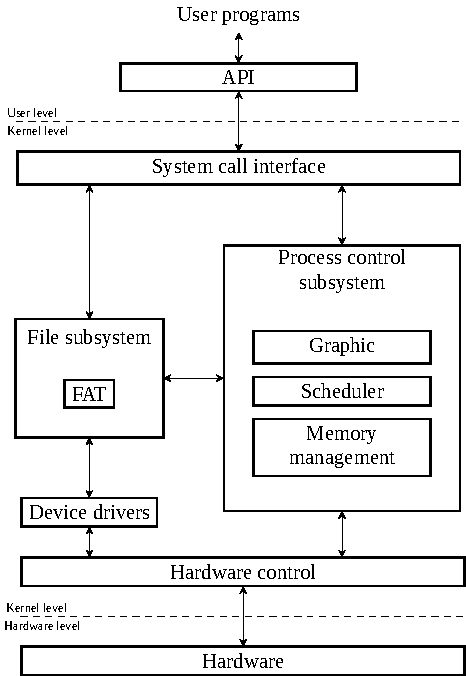
\includegraphics[width=.7\textwidth]{kernel-block.pdf}
  \caption{Top-level design}
  \label{fig:top-level}
\end{figure}


\section{Detailed Design}
\label{sec:detailed-design}

This section discusses the system design in details, including the function of each
module, data structures used in boot loader, kernel, API, and APPs.

\subsection{Boot Up}
\label{sec:boot-up}

At this stage the boot loader loads the operating system kernel into memory. This is done
in the following four steps:
\begin{enumerate}
\item Display boot information;
\item Read the second sector;
\item Read two sides of a track;
\item Read the next cylinder until all twenty cylinders have been read.
\end{enumerate}

At this stage, it is also necessary to complete the 32-bit protection mode switch and jump
to the entry point of the operating system.

\subsection{Kernel}
\label{sec:kernel}

The kernel receives the API calls from user processes, and operates the
hardwares through the device drivers.\fxerror{say some more.}

\subsubsection{Memory Management}
\label{sec:memory-management-1}

The process may request memory space while running. When it is finished running, the
operating system kernel shall reclaim its memory space. % So the operating system should be
% able to manage memory. Memory utilization should be improved when managing memory.
\fxerror{say some more. you can get some ideas from wikipedia.}

\paragraph{Data Structures used in MM}

\begin{codeblock}[1]
\begin{ccode}
struct FREEINFO
{ 
  unsigned int addr; /* start address of free space */
  unsigned int size; /* size of free mem in bytes*/
};
\end{ccode}
\end{codeblock}
\begin{itemize}
\item % (Code~\ref{src:FREEINFO})
  is used to record the size in bytes of free memory while
  the system is running.
\end{itemize}

\begin{codeblock}[1]
\begin{ccode}
struct MEMMAN
{ 
  int frees;    /* free memory blocks */
  int maxfrees; /* max of frees */
  int lostsize; /* release the sum of the failed memory size ??????????*/
  int losts;    /* number of failures */
  struct FREEINFO free[MEMMAN_FREES]; /* free memory block info */
};
\end{ccode}
\end{codeblock}
\begin{itemize}
\item is used to record the entire
memory usage, such as the total remaining free memory space and \fxerror*{???}{entries}.
\end{itemize}

\paragraph{Memory Management Functions}

\begin{ccode}
void memman_init(struct MEMMAN* man);
\end{ccode}
\begin{itemize}
\item The memory space is initialized and the \texttt{man} variable is used to record the
  memory space usage and free information.
\end{itemize}

\begin{ccode}
unsigned int memman_total(struct MEMMAN* man);
\end{ccode}
\begin{itemize}
\item Report the sum of all empty space. Return the size of free memory.
\end{itemize}

\begin{ccode}
unsigned int memman_alloc(struct MEMMAN *man, unsigned int size);
\end{ccode}
\begin{itemize}
\item Allocate memory to the application, where \texttt{size} is the space requested by the
  application. Success returns the available starting address, otherwise 0.
\end{itemize}

\begin{ccode}
int memman_free(struct MEMMAN *man, unsigned int addr, unsigned int size);
\end{ccode}
\begin{itemize}
\item Releases memory, where \texttt{addr} is the starting address variable and
  \texttt{size} is the size of the release variable. Returns 0 if successful, otherwise
  -1.
\end{itemize}

\begin{ccode}
unsigned int memman_alloc_4k(struct MEMMAN *man, unsigned int size);
\end{ccode}
\begin{itemize}
\item Memory is allocated in 4k memory units and the starting address of the allocated
  memory is returned. \texttt{size} is the size of requested space.
\end{itemize}

\begin{ccode}
int memman_free_4k(struct MEMMAN *man, unsigned int addr, unsigned int size);
\end{ccode}
\begin{itemize}
\item Memory space is freed in units of 4k, \texttt{addr} is the starting
  point variable, and \texttt{size} is the release size.
\end{itemize}

\subsubsection{Task Management (Scheduler)}
\label{sec:task-management}

The general operating systems need to be able to support multitasking. Simply saying that
multi-tasking is running multiple programs at the same time. But this only gives the user
an illusion. For a single CPU, it cannot handle multiple programs at the same time. It
merely divides the CPU time into many small pieces for different programs to run. The
operating system should be able to do task switching, that is to pass the CPU from one
process to another. And at a later time to switch it back, as shown in
Fig.~\ref{fig:ctxt-switch}. \fxerror*{see wikipedia}{Therefore, the register values should
  be saved when the task is switched. The task switching itself also takes time. The
  operating system should try to shorten this time. Doing this on the one hand provides
  the user with a good experience and does not leave the user with a delayed
  impression. On the other hand, reducing this time can improve CPU utilization. Because
  this time can not be used for program operation.}

\begin{figure}
  \centering
  \begin{center}
    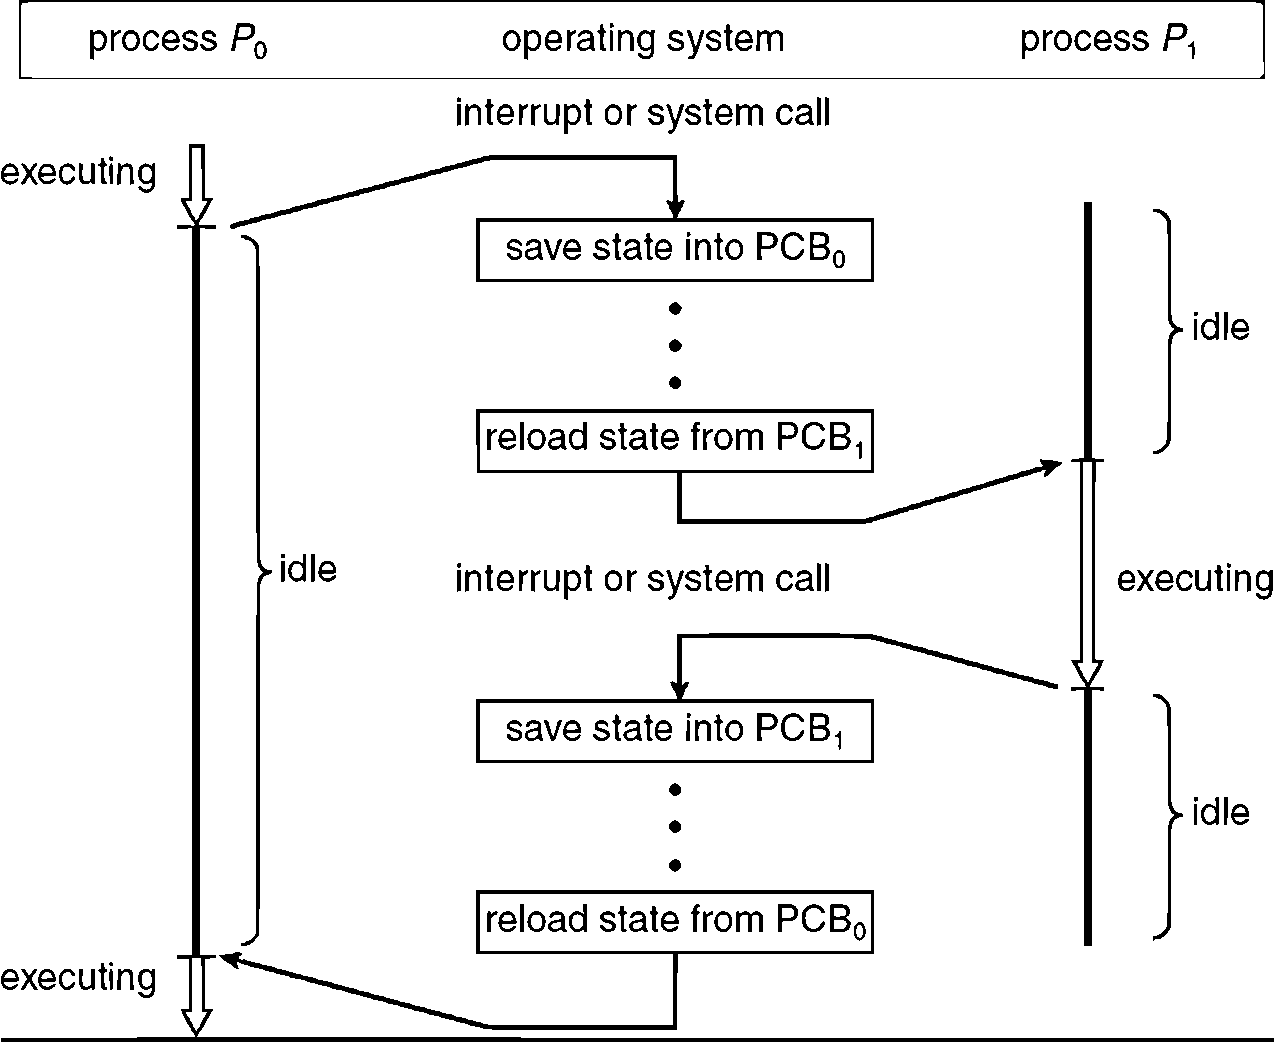
\includegraphics[width=.5\textwidth]{switch}
  \end{center}
  \caption{Context switch}
  \label{fig:ctxt-switch}
\end{figure}

\paragraph{Data Structures For Task Management}

\begin{codeblock}[1]
\begin{ccode}
struct TASKLEVEL
{ 
  int running; /* how many tasks are running */
  int now;     /* which task is currently running */
  struct TASK* tasks[MAX_TASKS_LV]; /* all tasks in one level */
};
\end{ccode}
\end{codeblock}
\begin{itemize}
\item is used to record the status of each task in a layer\fxerror{What's a layer/level?}.
\end{itemize}

\begin{codeblock}[1]
\begin{ccode}
struct TSS32
{ 
  int esp0, esp1, esp2; /* stack pointer register */
  int ss0, ss1, ss2;    /* stack segment register */
  int cr3;    /* control register */
  int eip;    /* instruct pointer register */
  int eflags; /* registers flag */
  int eax;    /* accumulator register */
  int ecx;    /* counter register */
  int edx;    /* data register */
  int ebx;    /* base register */
  int esp;    /* stack pointer register */
  int ebp;    /* base pointer register*/
  int esi;    /* source index register */
  int edi;    /* destination index register */
  int es;     /* extra segment register */
  int cs;     /* code segment register */
  int ss;     /* stack segment register */
  int ds;     /* data segment register */
  int fs;     /* segment part 2 */
  int gs;     /* segment part 3 */
  int ldtr;   /* LDT segment selector */
  int iomap;  /* I/O map base address */
};
\end{ccode}
\end{codeblock}
\begin{itemize}
\item holds information about task status segments, which are based on CPU
  specifications\cite[Sec.6.2.1]{intel_3a}.
\end{itemize}

\begin{codeblock}[1]
\begin{ccode}
struct TASKCTL
{ 
  int now_lv;    /* current activity level */
  int lv_change; /* does the hierarchy need to be changed next time the task is switched */
  struct TASKLEVEL level[MAX_TASKLEVELS]; /* all levels*/
  struct TASK tasks0[MAX_TASKS];          /* all running program */
};
\end{ccode}
\end{codeblock}
\begin{itemize}
\item is used to control all tasks in the system.\fxerror{not clear.}
\end{itemize}

\begin{codeblock}[1]
\begin{ccode}
struct TASK
{ 
  int sel;              /* the number of GDT */
  int flags;            /* the state of task */
  int level;            /* the level of task */
  int priority;         /* the priority of task */
  struct FIFO32 fifo;   /* a fifo buffer */
  TSS32 tss;            /* TSS segment for a task */
  struct CONSOLE* cons; /* the console window address of task */
  int ds_base;          /* data segment address of APPs */
  int cons_stack;       /* the stack address of APPs */
  struct SEGMENT_DESCRIPTOR ldt[2]; /* tow LDT segments of task */
  struct FILEHANDLE* fhandle; /* file handles for manipulating files */
  int* fat; /* file allocation table */
  char* cmdline; /* store the command line context */
  unsigned char langmode;  /* which font to use */
  unsigned char langbyte1; /* store the first byte of the full-width character */
};
\end{ccode}
\end{codeblock}
\begin{itemize}
\item is used to manage variables for a task. Record the task's sections, permissions,
  stacks, etc.
\end{itemize}

\paragraph{Task Management Functions}

\begin{ccode}
struct TASK *task_now(void);
\end{ccode}
\begin{itemize}
\item Returns which level of which task is currently running.
\end{itemize}

\begin{ccode}
struct TASK *task_init(struct MEMMAN *memman);
\end{ccode}
\begin{itemize}
\item Initialize a task.
\end{itemize}

\begin{ccode}
struct TASK *task_alloc(void);
\end{ccode}
\begin{itemize}
\item Initialize the structure of a task.
\end{itemize}

\begin{ccode}
void task_run(struct TASK *task, int level, int priority);
\end{ccode}
\begin{itemize}
\item Add a task to list.
\end{itemize}

\begin{ccode}
void task_switch(void);
\end{ccode}
\begin{itemize}
\item Switch to the next task.
\end{itemize}

\begin{ccode}
void task_sleep(struct TASK *task);
\end{ccode}
\begin{itemize}
\item Put a task to sleep.
\end{itemize}

\subsubsection{Graphic Management}
\label{sec:graphic}

The patterns on the screen belong to one layer. The movement of the window is achieved
through layers\fxerror{???}. The height of the layer affects the layout of the
screen. \fxerror*{bad}{Layers to consider how to cover when moving, which one is on and
  below.}
  
\paragraph{Graphic Management Data Structures}

\begin{codeblock}[1]
\begin{ccode}
struct SHEET
{ 
  char* buf;   /* address of the graphic content depicted */
  int bxszie;  /* size of x coordinate of sheet */
  int bysize;  /* size of y coordinate of sheet */
  int vx0;     /* x coordinate of sheet */
  int vy0;     /* y coordinate of sheet */
  int col_inv; /* number of invisible color */
  int height;  /* height of sheet */
  int flags;   /* states of sheet, using or not */
};
\end{ccode}
\end{codeblock}
\begin{itemize}
\item is used to record layer-related information, including the layer's size and
  position.
\end{itemize}

\begin{codeblock}[1]
\begin{ccode}
struct SHTCTL
{ 
  unsigned char* vram; /* the address of VRAM */
  unsigned char* map;  /* which layer the pixel on the screen belongs to*/
  int xsize; /* the x size of screen */
  int ysize; /* the y size of screen */
  int top;   /* the height of the top layer */
  struct SHEET* sheets[MAX_SHEETS]; /* order all layer addresses in order */
  struct SHEET sheets0[MAX_SHEETS]; /* all layers */
};
\end{ccode}
\end{codeblock}
\begin{itemize}
\item is used to manage the structure of multiple layer information, including how many
  layers there are in total, the size and height of each layer.
\end{itemize}

\paragraph{Graphic Management Functions}

\begin{ccode}
struct SHTCTL *shtctl_init(struct MEMMAN *memman,unsigned char *vram,int xsize,int ysize);
\end{ccode}
\begin{itemize}
\item Initialize a sheet control structure, \texttt{vram} is the address of video
  RAM. \texttt{xsize} and \texttt{ysize} is the size of sheet.
\end{itemize}

\begin{ccode}
struct SHEET *sheet_alloc(struct SHTCTL *ctl);
\end{ccode}
\begin{itemize}
\item Return a \texttt{SHEET} structure if success, otherwise 0.
\end{itemize}

\begin{ccode}
void sheet_setbuf(struct SHEET *sht,unsigned char *buf,int xsize,int ysize,int col_inv);
\end{ccode}
\begin{itemize}
\item Set the properties of the layer \texttt{buf}.
\end{itemize}

\begin{ccode}
void sheet_updown(struct SHEET *sht, int height);
\end{ccode}
\begin{itemize}
\item Set the height of layer \texttt{sht}.
\end{itemize}

\begin{ccode}
void sheet_refresh(struct SHEET *sht, int bx0, int by0, int bx1, int by1);
\end{ccode}
\begin{itemize}
\item Refreshes the screen range specified by \texttt{bx0}, \texttt{by0}, \texttt{bx1} and
  \texttt{by1}.
\end{itemize}

\begin{ccode}
void sheet_free(struct SHEET *sht);
\end{ccode}
\begin{itemize}
\item Release layer.
\end{itemize}

\begin{ccode}
void make_window8(unsigned char *buf, int xsize, int ysize, char *title, char act);
\end{ccode}
\begin{itemize}
\item Make a window in \texttt{SHEET} \texttt{buf}.
\end{itemize}

\begin{ccode}
void putfonts8_asc_sht(struct SHEET *sht, int x, int y, int c, int b, char *s, int l);
\end{ccode}
\begin{itemize}
\item Paint the background color and write the characters and finish the refresh.
\end{itemize}

\subsubsection{System Calls}
\label{sec:system-call}

The system calls encapsulate each module in the kernel\fxerror{???}. These system calls are part of the
kernel. In this system, system calls are called by the API instead of the
application.\fxerror{see wikipedia}

\paragraph{System Calls Prototype}

\begin{ccode}
void cons_putchar(struct CONSOLE *cons, int chr, char move);
\end{ccode}
\begin{itemize}
\item put a \texttt{chr} character on \texttt{cons} console.
\end{itemize}

\begin{ccode}
void cons_newline(struct CONSOLE *cons);
\end{ccode}
\begin{itemize}
\item newline in \texttt{cons} console.
\end{itemize}

\begin{ccode}
void cons_putstr0(struct CONSOLE *cons, char *s);
\end{ccode}
\begin{itemize}
\item put string \texttt{s} in \texttt{cons} console, no length.
\end{itemize}

\begin{ccode}
void cons_putstr1(struct CONSOLE *cons, char *s, int l);
\end{ccode}
\begin{itemize}
\item put string \texttt{s} in \texttt{cons}, \texttt{l} is the length of string
  \texttt{s}.
\end{itemize}

\begin{ccode}
int cmd_app(struct CONSOLE *cons, int *fat, char *cmdline);
\end{ccode}
\begin{itemize}
\item Start an application based on the input from the command line \texttt{cmdline};
\end{itemize}

\subsubsection{Driver}
\label{sec:driver}

The device drivers are used to control and manipulate the
hardware. \fxerror*{wikipedia}{The driver blocked the hardware information}. It is the
dividing line between hardware and software. A driver provides a software interface to
hardware devices, enabling operating systems and other computer programs to access
hardware functions without needing to know precise details of the hardware being used.

\paragraph{Driver Functions}

\begin{ccode}
void set_palette(int start, int end, unsigned char *rgb);
\end{ccode}
\begin{itemize}
\item initialize the palette.
\end{itemize}

\begin{ccode}
void init_pic(void);
\end{ccode}
\begin{itemize}
\item initialize the PIC.
\end{itemize}

\begin{ccode}
void init_keyboard(struct FIFO32 *fifo, int data0);
\end{ccode}
\begin{itemize}
\item initialze the keyboard.
\end{itemize}

\begin{ccode}
void enable_mouse(struct FIFO32 *fifo, int data0, struct MOUSE_DEC *mdec);
\end{ccode}
\begin{itemize}
\item activate mouse.
\end{itemize}

\subsubsection{FAT File System}
\label{sec:fat}

\fxerror*{wikipedia}{The file system defines how data is stored and accessed. The file
  system divides the entire storage space according to a certain form. This facilitates
  the storage of files while increasing the utilization of storage media. The small blocks
  thus divided are called sectors. The FAT records which sectors all files are stored on.}
  
\paragraph{FAT Data Structure}

\begin{codeblock}[1]
\begin{ccode}
struct FILEINFO
{ 
  unsigned char name[8];   /* file name */
  unsigned char ext[3];    /* extend name of file */
  unsigned char type;      /* file attributes */
  char reserve[10];        /* reserve byte */
  unsigned short time;     /* the time for storing file */
  unsigned short date;     /* the date for storing file */
  unsigned short  clustno; /* the file from which sector on the disk is stored */
};
\end{ccode}
\end{codeblock}
\begin{itemize}
\item is used to record file-related information, such as file name, size, etc.
\end{itemize}

\paragraph{FAT Functions}

\begin{ccode}
void file_readfat(int *fat, unsigned char *img);
\end{ccode}
\begin{itemize}
\item read file allocation table
\end{itemize}

\begin{ccode}
void file_loadfile(int clustno, int size, char *buf, int *fat, char *img);
\end{ccode}
\begin{itemize}
\item read file contents into memory
\end{itemize}


\begin{ccode}
struct FILEINFO *file_search(char *name, struct FILEINFO *finfo, int max);
\end{ccode}
\begin{itemize}
\item search for files based on provided \texttt{name}.
\end{itemize}


\subsection{API}
\label{sec:api}
In computer programming, APIs are subroutines that are used to develop
applications. Usually, it communicates all parts of the software. A good API makes
application development easier. By abstracting the underlying implementation and only
exposing objects or actions the developer needs, an API simplifies programming.

\subsubsection{All APIs}
\label{sec:all-apis}


\begin{ccode}
void api_putchar(int c);
\end{ccode}
\begin{itemize}
\item output a character \texttt{c} on the console window.
\end{itemize}



\begin{ccode}
void api_putstr0(char *s);
\end{ccode}
\begin{itemize}
\item ouput a string \texttt{s} on the console window.
\end{itemize}



\begin{ccode}
void api_putstr1(char *s, int l);
\end{ccode}
\begin{itemize}
\item output a string \texttt{s} on console window, \texttt{l} is the length of this string.
\end{itemize}


\begin{ccode}
void api_end(void);
\end{ccode}
\begin{itemize}
\item end the application's running.
\end{itemize}


\begin{ccode}
int api_openwin(char *buf, int xsiz, int ysiz, int col_inv, char *title);
\end{ccode}
\begin{itemize}
\item open a window, return the hanlder of window.
\end{itemize}


\begin{ccode}
void api_putstrwin(int win, int x, int y, int col, int len, char *str);
\end{ccode}
\begin{itemize}
\item display string \texttt{str} on window. 
\end{itemize}



\begin{ccode}
void api_boxfilwin(int win, int x0, int y0, int x1, int y1, int col);
\end{ccode}
\begin{itemize}
\item draw a box on the window
\end{itemize}



\begin{ccode}
void api_initmalloc(void);
\end{ccode}
\begin{itemize}
\item initialize the structure of the management memory
\end{itemize}



\begin{ccode}
char *api_malloc(int size);
\end{ccode}
\begin{itemize}
\item allocating memory for the application.
\end{itemize}



\begin{ccode}
void api_free(char *addr, int size);
\end{ccode}
\begin{itemize}
\item free up memory used by the application.
\end{itemize}



\begin{ccode}
void api_point(int win, int x, int y, int col);
\end{ccode}
\begin{itemize}
\item draw a pint on \texttt{win} window.
\end{itemize}



\begin{ccode}
void api_refreshwin(int win, int x0, int y0, int x1, int y1);
\end{ccode}
\begin{itemize}
\item refresh the window.
\end{itemize}



\begin{ccode}
void api_linewin(int win, int x0, int y0, int x1, int y1, int col);
\end{ccode}
\begin{itemize}
\item draw a straight line.
\end{itemize}


\begin{ccode}
void api_closewin(int win);
\end{ccode}
\begin{itemize}
\item close window.
\end{itemize}


\begin{ccode}
int api_getkey(int mode);
\end{ccode}
\begin{itemize}
\item accept keyboard input.
\end{itemize}


\begin{ccode}
int api_alloctimer(void);
\end{ccode}
\begin{itemize}
\item get timer.
\end{itemize}



\begin{ccode}
void api_inittimer(int timer, int data);
\end{ccode}
\begin{itemize}
\item set the data of timer sending.
\end{itemize}


\begin{ccode}
void api_settimer(int timer, int time);
\end{ccode}
\begin{itemize}
\item set the time of timer.
\end{itemize}



\begin{ccode}
void api_freetimer(int timer);
\end{ccode}
\begin{itemize}
\item release timer.
\end{itemize}




\begin{ccode}
void api_beep(int tone);
\end{ccode}
\begin{itemize}
\item make a buzzer sound
\end{itemize}



\begin{ccode}
int api_fopen(char *fname);
\end{ccode}
\begin{itemize}
\item open file, return file hanlder
\end{itemize}



\begin{ccode}
void api_fclose(int fhandle);
\end{ccode}
\begin{itemize}
\item close file
\end{itemize}


\begin{ccode}
void api_fseek(int fhandle, int offset, int mode);
\end{ccode}
\begin{itemize}
\item locate a file
\end{itemize}



\begin{ccode}
int api_fsize(int fhandle, int mode);
\end{ccode}
\begin{itemize}
\item return the size of \texttt{fhandle} file.
\end{itemize}



\begin{ccode}
int api_fread(char *buf, int maxsize, int fhandle);
\end{ccode}
\begin{itemize}
\item read file, return read bytes. 
\end{itemize}



\begin{ccode}
int api_cmdline(char *buf, int maxsize);
\end{ccode}
\begin{itemize}
\item return the context of command line.
\end{itemize}



\begin{ccode}
int api_getlang(void);
\end{ccode}
\begin{itemize}
\item return the language mode.
\end{itemize}



\subsection{APPs}
\label{sec:apps-1}
Since this design is only about the operating system itself, only three representative
applications are introduced. The first is the application of the display color:
\texttt{color}. The second is the application for timing: \texttt{sundial}. The third
application is to imitate the application of stars in the sky: \texttt{stars2}.

\iffalse %%%%%%%%%%%%%%%%%%%%%%%%%%%%%%%%%%%%%%%%%%%%%%%%%%%%%%%%%%%%%%%%%%%%%%%%%%%%%%%%%%%%%%%%%%
\subsubsection{1. Data Structure in Kernel}
In this section data structures used in the RongOS operating system will be introduced in
detail.

\paragraph{BOOTINFO}

\begin{listing}[H]
  \begin{codeblock}
\begin{ccode}
struct BOOTINFO
{
  char cyls;          /* how many cylinder should be read */
  char leds;          /* the status of LED on keyboard */
  char vmode;         /* the mode of video card */
  char reserve;
  short scrnx, scrny; /* resolution of screen */
  char *vram;
};
\end{ccode}
  \end{codeblock}
  \caption{\texttt{struct BOOTINFO}}\label{src:bootinfo}
\end{listing}

(code~\ref{src:bootinfo}) is used to store startup-related
information, such as how many cylinders were read, the status of the keyboard indicator,
the mode of the screen, the size of the screen, and the memory address of the graphics
card.


\paragraph{FIFO32}

\begin{listing}[H]
  \begin{codeblock}
\begin{ccode}
struct 
{ 
  int* buf;          /* the address of FIFO32 buffer */
  int p;             /* the writing address */
  int q;             /* the reading address */
  int size;          /* the size of FIFO32 buffer */
  int free;          /* how many space free */
  int flags;         /* the states of FIFO32 buffer */
  struct TASK* task; /* point to a task */ 
};
\end{ccode}
  \end{codeblock}
  \caption{\texttt{struct FIFO32}}\label{src:FIFO32}
\end{listing}

(code~\ref{src:FIFO32}) is used to
describe a FIFO structure. This structure is used to receive various kinds of
information. It specifies where to read and write the FIFO structure and the size of the
buffer, available size.


\paragraph{SEGMENT\_DESCRIPTOR}

\begin{listing}[H]
  \begin{codeblock}
\begin{ccode}
struct 
{ 
  short limit_low;   /* the low part of segment size */
  short base_low;    /* the low part of base address */
  char base_mid;     /* the middle part of base address */
  char access_right; /* read and write permissions etc */
  char  limit_high;  /* the high part of segment size */
  char base_high;    /* the high part of base address */
};
\end{ccode}
  \end{codeblock}
  \caption{\texttt{struct SEGMENT\_DESCRIPTOR}}\label{src:DESCRIPTOR}
\end{listing}

(code~\ref{src:DESCRIPTOR}) structure is
used to store GDT related information, which is based on CPU specifications(3.5.1 and
3.4.5\cite{intel_3a}). GDT is stored at 270000 in memory.


\paragraph{GATE\_DESCRIPTOR}

\begin{listing}[H]
  \begin{codeblock}
\begin{ccode}
struct 
{ 
  short offset_low;   /* the low part of offset */
  short selector;     /* which interrupt to choose */
  char dw_count;      /* how many interrupts are registered */
  char access_right;  /* access permission */
  short  offset_high; /* high part of offset */
};
\end{ccode}
  \end{codeblock}
  \caption{\texttt{struct GATE\_DESCRIPTOR}}\label{src:GATEDESCRIPTOR}
\end{listing}

(code~\ref{src:GATEDESCRIPTOR}) structure is used to
store IDT related information, which is based on CPU specifications(3.5.1 and
3.4.5\cite{intel_3a}). IDT is at 26f800 memory.


\paragraph{MOUSE\_DEC}

\begin{listing}[H]
  \begin{codeblock}
\begin{ccode}
struct 
{ 
  unsigned char buf[3]; /* store the data from mouse */
  unsigned char phase;  /* the stage of receiving mouse data */
  int x;                /* the x point of mouse */
  int y;                /* the y point of mouse */
  int btn;              /* whether the mouse is pressed */
};
\end{ccode}
  \end{codeblock}
  \caption{\texttt{struct MOUSE\_DEC}}\label{src:MOUSE}
\end{listing}

(code~\ref{src:MOUSE}) structure is used to store information about the mouse, such as the
location of the mouse, whether the mouse is pressed or not.

\paragraph{FREEINFO}

\begin{listing}[H]
  \begin{codeblock}
\begin{ccode}
struct 
{ 
  unsigned int addr; /* the starting address of free space */
  unsigned int size; /* how many size is free */
};
\end{ccode}
  \end{codeblock}
  \caption{\texttt{struct FREEINFO}}\label{src:FREEINFO}
\end{listing}

(code~\ref{src:FREEINFO}) structure stores how many bytes are
free from where in memory.




\paragraph{MEMMAN}

\begin{listing}[H]
  \begin{codeblock}
\begin{ccode}
struct 
{ 
  int frees;                           /* how many memory blocks are free */
  int maxfrees;                        /* the maximum of frees */
  int lostsize;                        /* release the sum of the failed memory size */
  int losts;                           /* the number of failures */
  struct FREEINFO free[MEMMAN_FREES];  /* record all free memory block information */
};
\end{ccode}
  \end{codeblock}
  \caption{\texttt{struct MEMMAN}}\label{src:MEMMAN}
\end{listing}

(code~\ref{src:MEMMAN}) structure is used to store the entire memory usage, such as the total
remaining memory space and entries.



\paragraph{SHEET}

\begin{listing}[H]
  \begin{codeblock}
\begin{ccode}
struct 
{ 
  char* buf;   /* the address of the graphic content depicted */
  int bxszie;  /* the size of x coordinate of sheet */
  int bysize;  /* the size of y coordinate of sheet */
  int vx0;     /* the x coordinate of sheet */
  int vy0;     /* the y coordinate of sheet */
  int col_inv; /* the number of invisible color */
  int height;  /* the height of sheet */
  int flags;   /* the states of sheet, using or not */
};
\end{ccode}
  \end{codeblock}
  \caption{\texttt{struct SHEET}}\label{src:SHEET}
\end{listing}

(code~\ref{src:SHEET}) structure is used to store the entire memory usage, such as the
total remaining memory space and entries.



\paragraph{SHTCTL}

\begin{listing}[H]
  \begin{codeblock}
\begin{ccode}
struct 
{ 
  unsigned char* vram;              /* the address of VRAM */
  unsigned char* map;               /* which layer the pixel on the screen belongs to*/
  int xsize;                        /* the x size of screen */
  int ysize;                        /* the y size of screen */
  int top;                          /* the height of the top layer */
  struct SHEET* sheets[MAX_SHEETS]; /* order all layer addresses in order */
  struct SHEET sheets0[MAX_SHEETS]; /* all layers */
};
\end{ccode}
  \end{codeblock}
  \caption{\texttt{struct SHTCTL}}\label{src:SHTCTL}
\end{listing}

(code~\ref{src:SHTCTL}) structure is used to manage the structure of multiple layer information,
including how many layers there are in total, the size and height of each layer.



\paragraph{TIMER}

\begin{listing}[H]
  \begin{codeblock}
\begin{ccode}
struct 
{ 
  struct TIMER* next;   /* the next timer that is about to timeout */
  unsigned int timeout; /* how long is the timeout */
  char flags;           /* the states of timer */
  char flgas2;          /* whether to allow automatic cancellation */
  struct FIFO32* fifo;  /* store data(from mouse, keyboard etc) */
  int data;             /* accept data */
};
\end{ccode}
  \end{codeblock}
  \caption{\texttt{struct TIMER}}\label{src:TIMER}
\end{listing}

(code~\ref{src:TIMER}) structure is used to manage the time slice of the CPU. The timer
interrupts the CPU at regular intervals. This structure records the length of the timer,
usage status and other information.



\paragraph{TIMERCTL}

\begin{listing}[H]
  \begin{codeblock}
\begin{ccode}
struct 
{ 
  unsigned int count;   /* count variable */
  unsigned int next;    /* the next timeout timer */
  sturct TIMER* t0;     /* the shortest timeout timer */
  struct TIMER timers0; /* all timers */
};
\end{ccode}
  \end{codeblock}
  \caption{\texttt{struct TIMERCTL}}\label{src:TIMERCTL}
\end{listing}

(code~\ref{src:TIMERCTL}) structure is used to manage all timers in the system. Including
how many timers are in total, current use, and the next timer to be used.



\paragraph{TSS32}

\begin{listing}[H]
  \begin{codeblock}
\begin{ccode}
struct 
{ 
  int esp0, esp1, esp2; /* stack pointer register */
  int ss0, ss1, ss2;    /* stack segment register */
  int cr3;              /* control register */
  int eip;              /* instruct pointer register */
  int eflags;           /* registers flag */
  int eax;              /* accumulator register */
  int ecx;              /* counter register */
  int edx;              /* data register */
  int ebx;              /* base register */
  int esp;              /* stack pointer register */
  int ebp;              /* base pointer register*/
  int esi;              /* source index register */
  int edi;              /* destination index register */
  int es;               /* extra segment register */
  int cs;               /* code segment register */
  int ss;               /* stack segment register */
  int ds;               /* data segment register */
  int fs;               /* segment part 2 */
  int gs;               /* segment part 3 */
  int ldtr;             /* LDT segment selector */
  int iomap;            /* I/O map base address */
};
\end{ccode}
  \end{codeblock}
  \caption{\texttt{struct TSS32}}\label{src:TSS32}
\end{listing}

(code~\ref{src:TSS32}) structure holds information about task status segments, which are
based on CPU specifications(See 6.2.1\cite{intel_3a}).


\paragraph{FILEHANDLE}

\begin{listing}[H]
  \begin{codeblock}
\begin{ccode}
struct 
{ 
  char* buf; /* store the handler of file */
  int size;  /* the size of file */
  int pos;   /* where to read the file */
};
\end{ccode}
  \end{codeblock}
  \caption{\texttt{struct FILEHANDLE}}\label{src:FILEHANDLE}
\end{listing}

(code~\ref{src:FILEHANDLE}) is used to record an open file related data structure.



\paragraph{TASK}

\begin{listing}[H]
  \begin{codeblock}
\begin{ccode}
struct 
{ 
  int sel;                          /* the number of GDT */
  int flags;                        /* the state of task */
  int level;                        /* the level of task */
  int priority;                     /* the priority of task */
  struct FIFO32 fifo;               /* a fifo buffer */
  TSS32 tss;                        /* TSS segment for a task */
  struct CONSOLE* cons;             /* the console window address of task */
  int ds_base;                      /* data segment address of APPs */
  int cons_stack;                   /* the stack address of APPs */
  struct SEGMENT_DESCRIPTOR ldt[2]; /* tow LDT segments of task */
  struct FILEHANDLE* fhandle;       /* file handles for manipulating files */
  int* fat;                         /* file allocation table */
  char* cmdline;                    /* store the command line context */
  unsigned char langmode;           /* which font to use */
  unsigned char langbyte1;          /* store the first byte of the full-width character */
};
\end{ccode}
  \end{codeblock}
  \caption{\texttt{struct TASK}}\label{src:TASK}
\end{listing}

(code~\ref{src:TASK})is used to manage variables for a task. Record the task's sections,
permissions, stacks, etc.


\paragraph{TASKLEVEL}

\begin{listing}[H]
  \begin{codeblock}
\begin{ccode}
struct 
{ 
  int running;                      /* how many tasks are running */
  int now;                          /* which task is currently running */
  struct TASK* tasks[MAX_TASKS_LV]; /* all tasks in one level */
};
\end{ccode}
  \end{codeblock}
  \caption{\texttt{struct TASKLEVEL}}\label{src:TASKLEV}
\end{listing}

(code~\ref{src:TASKLEV}) is used to record the status of each task in a layer.


\paragraph{TASKCTL}

\begin{listing}[H]
  \begin{codeblock}
\begin{ccode}
struct 
{ 
  int now_lv;    /* current activity level */
  int lv_change; /* does the hierarchy need to be changed next time the task is switched */
};
\end{ccode}
  \end{codeblock}
  \caption{\texttt{struct TASKCTL}}\label{src:TASKCT}
\end{listing}

(code~\ref{src:TASKCT}) is used to control all tasks in the system.



\paragraph{CONSOLE}

\begin{listing}[H]
  \begin{codeblock}
\begin{ccode}
struct 
{ 
  struct SHEET* sht;   /* which layer is used on the command line */
  int cur_x;           /* the x position of console */
  int cur_y;           /* the y position of console */
  int cur_c;           /* the color of console */
  struct TIMER* timer; /* timer to control cursor blinking */
};
\end{ccode}
  \end{codeblock}
  \caption{\texttt{struct CONSOLE}}\label{src:CONSOLE}
\end{listing}

(code~\ref{src:CONSOLE})is used to record information about a console terminal, such as location,
color, and so on.




\paragraph{FILEINFO}

\begin{listing}[H]
  \begin{codeblock}
\begin{ccode}
struct 
{ 
  unsigned char name[8];   /* file name */
  unsigned char ext[3];    /* extend name of file */
  unsigned char type;      /* file attributes */
  char reserve[10];        /* reserve byte */
  unsigned short time;     /* the time for storing file */
  unsigned short date;     /* the date for storing file */
  unsigned short  clustno; /* the file from which sector on the disk is stored */
};
\end{ccode}
  \end{codeblock}
  \caption{\texttt{struct FILEINFO}}\label{src:FILEINFO}
\end{listing}

(code~\ref{src:FILEINFO}) is used to record file-related information, such as file name, size,
etc.
\fi %%%%%%%%%%%%%%%%%%%%%%%%%%%%%%%%%%%%%%%%%%%%%%%%%%%%%%%%%%%%%%%%%%%%%%%%%%%%%%%%%%%%%%%%%%%%%%%%%%%%%%%


    
%\subsection{API}
%\label{sec:api}

%\subsection{APPs}
%\label{sec:apps-1}



\chapter{Implementation}

\section{Boot Up}
\label{sec:boot-up-1}

The boot loader is implemented in Intel assembly. It works as follows:

\begin{enumerate}
\item \textbf{Display boot information:} Firstly, the code in boot sector (See
  Appendix~\ref{sec:dis-boo-inf}) outputs some boot information. \fxerror*{Not clear. You
    have to explain what is al/ah for. For example, as shown in table... al is for..., ah
    is for... int 0x10 is for...}{When \texttt{al=0}, the
  null character of boot information hit. Interrupt \texttt{0x10} is used for showing a
  character on the screen.}
\item \textbf{Read the second sector:} Then jump to load C0-H0-S2, \texttt{ax} register
  saved the address where beginning puts the sectors from floppy. And preparing parameters
  for interrupt \texttt{0x13} in registers. The \texttt{0x13} interrupt used for read
  sector from floppy to memory. (See Appendix~\ref{sec:rea-sec-sec}).
\item \textbf{Read two sides of a track:}
  
  If there is a carry indicating some thing went wrong while reading the floppy disk,
  reset the registers and try reading it again. The read process aborts after five
  unsuccessful read.

  Register \texttt{si} is a counter. If no carry (success), jump to next segment, as one
  sector has been read into memory already. The address should increase 512 byte. Then
  sector number (\texttt{cl} register) is added by 1 and compare it to 18, if it's smaller
  than 18, jump to \texttt{readloop}, read the next sector.

  If the value of \texttt{cl} register is bigger or equal to 18, meaning that one track
  18 sector in this side of floppy read already, then reversed the head, add 1 to
  \texttt{dh} register.

  If the value of \texttt{dh} register after adding larger than or equal to 2, it's saying
  the original head is 1, one track of two sides read already. Otherwise the value of
  \texttt{dh} register smaller than 2, read this side indicating by \texttt{dh} register,
  jump to \texttt{readloop} segmentation. Appendix~\ref{sec:rea-two-sid} is the code 
  performing this function.

  There is a pseudo code about this process:
  \begin{figure}[!ht]
    \centering
    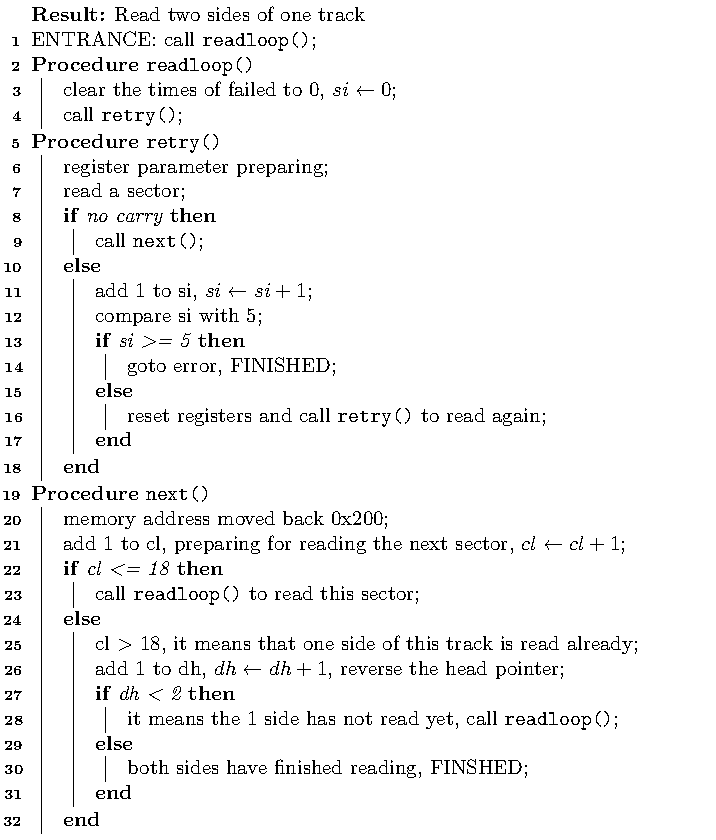
\includegraphics[width=.7\textwidth]{./figs/algorithm/read_two_side.pdf}
    \label{fig:read_two_sides}
  \end{figure}

  
  
\item \textbf{The next cylinder:} So the next step is moving a cylinder, add 1 to register
  \texttt{ch}. Otherwise the value of \texttt{dh} register smaller than 2, read this side
  indicating by \texttt{dh} register, jump to \texttt{readloop} segmentation. After
  \texttt{ch} register add 1, if it's smaller than 10, jump to \texttt{readloop},
  otherwise end loading floppy to memory process, for we only load ten cylinders of
  floppy. Appendix~\ref{sec:the-nex-cyl} is the code to perform this function.
\end{enumerate}

The above four steps can be intuitively reflected in the Fig. ~\ref{fig:iplflowchart}.
\begin{figure}[!htbp]
  \centering
  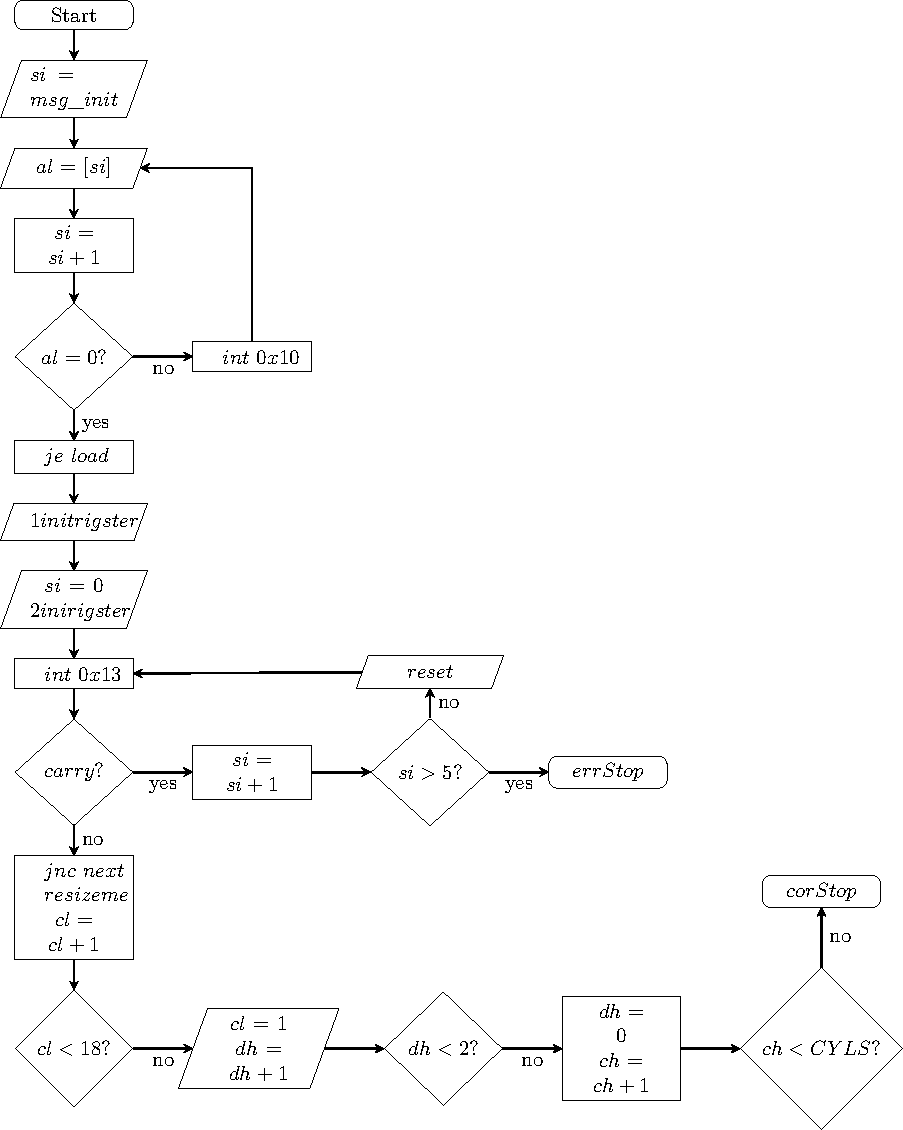
\includegraphics[width=1\textwidth]{flowchartp}
  \caption{the working flowchart of boot loader}
  \label{fig:iplflowchart}
\end{figure}

\section{Kernel}
\label{sec:kernel-1}



\section{API}
\label{sec:API}


\section{APPs}
\label{sec:apps}




\chapter{Conclusions}%{Prospects And Shortages}

\footnotetext{\url{https://thesistips.wordpress.com/2012/03/25/how-to-write-your-introduction-abstract-and-summary/}}

\paragraph{What goes in your ``Conclusions'' chapter?}

{\fontspec[Scale=.8]{Purisa} The purpose of this chapter is to provide a summary of the
  whole thesis or report.  In this context, it is similar to the Abstract, except that the
  Abstract puts roughly equal weight on all thesis/report chapters, whereas the
  Conclusions chapter focuses primarily on the findings, conclusions and/or
  recommendations of the project.

  There are a couple of rules – one rigid, one common sense, for this chapter:
  \begin{itemize}
  \item All material presented in this chapter must have appeared already in the report;
    no new material can be introduced in this chapter. (rigid rule of technical writing)
  \item Usually, you would not present any new figures or tables in this chapter. (rule of thumb)
  \end{itemize}

  Generally, for most technical reports and Masters theses, the Conclusions chapter would
  be~3 to 5 pages long (double spaced).  It would generally be longer in a large PhD
  thesis. Typically you would have a paragraph or two for each chapter or major
  subsection.  Aim to include the following (typical) content.
  \begin{enumerate}
  \item Re-introduce the project and the need for the work – though more briefly than in
    the intro;
  \item Re-iterate the purpose and specific objectives of your project.
  \item Re-cap the approach taken – similar to the road map in the intro; however, in this
    case, you are re-capping the data, methodology and results as you go.
  \item Summarize the major findings and recommendations of your work.
  \item Make recommendations for future research.
  \end{enumerate}}

%%% 正文部分到此结束。下面是『参考文献』、『指导教师简介』、『鸣谢』、『附录』

%% 不要动下面四行!
\appendix{}
\maketailpages{} % 参考文献、指导教师简介、鸣谢

%%% 下面是附录部分,可以没有。

\chapter{Main Program Code} %附录一

\section{Boot loader}

\subsection{Display boot information}
\label{sec:dis-boo-inf}

\inputminted[firstline=55, lastline=65,
linenos=true]{nasm}{../../src/kernel/ipl10.asm}

\subsection{Read the second sector}
\label{sec:rea-sec-sec}
  
\inputminted[firstline=87,lastline=106,linenos=true]{nasm}{../../src/kernel/ipl10.asm}

\subsection{Read two sides of a track}
\label{sec:rea-two-sid}

\inputminted[firstline=108,lastline=132,linenos=true]{nasm}{../../src/kernel/ipl10.asm}

\subsection{The next cylinder}
\label{sec:the-nex-cyl}

\inputminted[firstline=134,lastline=137,linenos=true]{nasm}{../../src/kernel/ipl10.asm}

\end{document} % 结束。不要动下面几行!

%%% Local Variables:
%%% mode: latex
%%% TeX-master: t
%%% End:
